\textbf{Pour chaque affirmation, répondre par VRAI ou FAUX, en justifiant la réponse.}

\medskip

\begin{minipage}[t]{0.58\linewidth}
	Au 1\up{er} janvier 2025, un étang contient \np{3000}~m$^3$ d'eau.

	Chaque année, l'étang perd 10\,\% de son volume d'eau.

	On modélise l'évolution du volume d'eau de cet étang par une suite $\left(u_n\right)$ où, pour tout entier naturel $n$, $u_n$ désigne la quantité d'eau, en mètre cube, contenue dans l'étang, le 1\up{er} janvier de l'année $2025+n$.

	Ainsi, on a $u_0 = \np{3000}$.

	La feuille de calcul ci-contre donne les valeurs des premiers termes de cette suite $\left(u_n\right)$.
\end{minipage}
\hfill
\begin{minipage}[t]{0.38\linewidth}
	\vspace{0pt}
	\begin{tikzpicture}[scale=0.62,transform shape]
		\tableur*[15]{A/2.5cm,B/2.5cm}
		\celtxt*[align=center]{A}{1}{$n$} \celtxt*[align=center]{B}{1}{$u_n$}
		\celtxt*[align=center]{A}{2}{$0$} \celtxt*[align=center]{B}{2}{$3000$}
		\celtxt*[align=center]{A}{3}{$1$} \celtxt*[align=center]{B}{3}{$2700$}
		\celtxt*[align=center]{A}{4}{$2$} \celtxt*[align=center]{B}{4}{$2430$}
		\celtxt*[align=center]{A}{5}{$3$} \celtxt*[align=center]{B}{5}{$2187$}
		\celtxt*[align=center]{A}{6}{$4$} \celtxt*[align=center]{B}{6}{$1968{,}3$}
		\celtxt*[align=center]{A}{7}{$5$} \celtxt*[align=center]{B}{7}{$1771{,}47$}
		\celtxt*[align=center]{A}{8}{$6$} \celtxt*[align=center]{B}{8}{$1594{,}323$}
		\celtxt*[align=center]{A}{9}{$7$} \celtxt*[align=center]{B}{9}{$1434{,}8907$}
		\celtxt*[align=center]{A}{10}{$8$} \celtxt*[align=center]{B}{10}{$1291{,}40163$}
		\celtxt*[align=center]{A}{11}{$9$} \celtxt*[align=center]{B}{11}{$1162{,}26147$}
		\celtxt*[align=center]{A}{12}{$10$} \celtxt*[align=center]{B}{12}{$1046{,}03532$}
		\celtxt*[align=center]{A}{13}{$11$} \celtxt*[align=center]{B}{13}{$941{,}431788$}
		\celtxt*[align=center]{A}{14}{$12$} \celtxt*[align=center]{B}{14}{$847{,}288609$}
		\celtxt*[align=center]{A}{15}{$13$} \celtxt*[align=center]{B}{15}{$762{,}559748$}
	\end{tikzpicture}
\end{minipage}

\begin{enumerate}
	\item \textbf{Affirmation}

	Pour obtenir les termes de la suite $\left(u_n\right)$, la formule saisie dans la cellule \textsf{B3} puis étirée vers le bas est : \fbox{\small\textsf{= 0,90 * A3}}

	\item \textbf{Affirmation}

	La suite $\left(u_n\right)$ est une suite arithmétique de raison $r = 0,90$ et de 1\up{er} terme $u_0 = \np{3000}$.
\end{enumerate}

\medskip

\begin{minipage}[t]{0.58\linewidth}
	Au 1\up{er} janvier 2025, un second étang contient quant à lui \np{4000}~m$^3$ d'eau. Chaque année, cet étang perd 20\,\% de son volume d'eau initial mais il est naturellement alimenté par un cours d'eau qui augmente son volume d'eau de 140~m$^3$ par an.

	On peut également modéliser l'évolution du volume d'eau de cet étang par une suite $\left(v_n\right)$ où, pour tout entier naturel $n$, $v_n$ désigne la quantité d'eau, en mètre cube, contenue dans l'étang, le 1\up{er} janvier de l'année $2025+n$.

	Ainsi, on a $v_0 = \np{4000}$.

	La feuille de calcul ci-contre donne les valeurs des premiers termes de cette suite $\left(v_n\right)$.
\end{minipage}
\hfill
\begin{minipage}[t]{0.38\linewidth}
	\vspace{0pt}
	\begin{tikzpicture}[scale=0.62,transform shape]
		\tableur*[15]{A/2.5cm,B/2.5cm}
		\fill[darkgray] (cellB-3.south west) rectangle (cellB-3.north east);
		\celtxt*[align=center]{A}{1}{$n$} \celtxt*[align=center]{B}{1}{$v_n$}
		\celtxt*[align=center]{A}{2}{$0$} \celtxt*[align=center]{B}{2}{$4000$}
		\celtxt*[align=center]{A}{3}{$1$}
		\celtxt*[align=center]{A}{4}{$2$} \celtxt*[align=center]{B}{4}{$2812$}
		\celtxt*[align=center]{A}{5}{$3$} \celtxt*[align=center]{B}{5}{$2389{,}6$}
		\celtxt*[align=center]{A}{6}{$4$} \celtxt*[align=center]{B}{6}{$2051{,}68$}
		\celtxt*[align=center]{A}{7}{$5$} \celtxt*[align=center]{B}{7}{$1781{,}344$}
		\celtxt*[align=center]{A}{8}{$6$} \celtxt*[align=center]{B}{8}{$1565{,}0752$}
		\celtxt*[align=center]{A}{9}{$7$} \celtxt*[align=center]{B}{9}{$1392{,}06016$}
		\celtxt*[align=center]{A}{10}{$8$} \celtxt*[align=center]{B}{10}{$1253{,}64813$}
		\celtxt*[align=center]{A}{11}{$9$} \celtxt*[align=center]{B}{11}{$1142{,}9185$}
		\celtxt*[align=center]{A}{12}{$10$} \celtxt*[align=center]{B}{12}{$1054{,}3348$}
		\celtxt*[align=center]{A}{13}{$11$} \celtxt*[align=center]{B}{13}{$983{,}467842$}
		\celtxt*[align=center]{A}{14}{$12$} \celtxt*[align=center]{B}{14}{$926{,}774273$}
		\celtxt*[align=center]{A}{15}{$13$} \celtxt*[align=center]{B}{15}{$881{,}419419$}
	\end{tikzpicture}
\end{minipage}

\begin{enumerate}[start=3]
	\item \textbf{Affirmation}

	On a $v_1 = \np{3340}$.

	\item \textbf{Affirmation}

	Les volumes des deux étangs passeront simultanément en dessous de \np{1000}~m$^3$ à partir de 2036.
\end{enumerate}

\medskip
